\documentclass{article}
\usepackage{graphicx,fancyhdr,amsmath,amssymb,amsthm,subfig,url}
\usepackage[margin=1in]{geometry}
\usepackage{setspace}
\usepackage{texs/tikzit}
\usepackage{pgfplots}
\input{texs/sample.tikzstyles}
\usepackage{enumitem}
\usepackage{array}   % for \newcolumntype macro
\usepackage{textcomp, gensymb}
\usepackage{cancel}
\usepackage{mathtools}

%----------------------- Macros and Definitions --------------------------
\renewcommand{\gcd}[1]{\text{gcd}\left(#1\right)}
\newcommand{\lcm}[1]{\text{lcm}\left(#1\right)}
\renewcommand{\min}[1]{\text{min}\left(#1\right)}
\renewcommand{\max}[1]{\text{max}\left(#1\right)}
\DeclarePairedDelimiter{\floor}{\lfloor}{\rfloor}
\renewcommand{\mod}[1]{\quad \left(\text{mod } #1\right)}
\newcommand{\vphi}[1]{\varphi(#1)}
\newcommand{\hrbar}{\scalebox{0.35}{\tikzfig{fig7_2}}}
\newcommand{\vrbar}{\scalebox{0.35}{\tikzfig{fig7_1}}}
\DeclarePairedDelimiter{\brf}{(}{)}
\newcolumntype{L}{>{$}l<{$}} % math-mode version of "l" column type

%%% FILL THIS OUT
\newcommand{\studentname}{Anwarul Bashir Shuaib}
\newcommand{\suid}{1805010}
\newcommand{\stampeq}{\stepcounter{equation} \tag{\theequation}}
%%% END



\renewcommand{\theenumi}{\bf \Alph{enumi}}

%\theoremstyle{plain}
%\newtheorem{theorem}{Theorem}
%\newtheorem{lemma}[theorem]{Lemma}

\fancypagestyle{plain}{}
\pagestyle{fancy}
\fancyhf{}
\fancyhead[RO,LE]{\sffamily\bfseries\large Mathematical Analysis for Computer Science}
\fancyhead[LO,RE]{\sffamily\bfseries\large CSE 301}
\fancyfoot[LO,RE]{\sffamily\bfseries\large \studentname: \suid @cse.buet.ac.bd}
\fancyfoot[RO,LE]{\sffamily\bfseries\thepage}
\renewcommand{\headrulewidth}{1pt}
\renewcommand{\footrulewidth}{1pt}

\graphicspath{{figures/}}

%-------------------------------- Title ----------------------------------

\title{CSE 301}
\author{\studentname \qquad Student ID: \suid}

%--------------------------------- Text ----------------------------------
\onehalfspacing
\setlength{\parindent}{0pt}
\begin{document}
\maketitle
\section*{Solution Outline:}
\begin{table}[h!]
    \centering
    \begin{tabular}{|c|c|c|c|c|}
        \hline
        Chapter      & Solved                                        & \#Solved & Unsolved         & \#Unsolved \\ \hline
        1            & 5, 6, 10, 11, 13, 14, 15, 19                  & 8        & 17, 21           & 2          \\ \hline
        2            & 11, 12, 14, 19, 20, 21, 22, 23, 24, 25 26, 29 & 12       & 13, 15, 30, 32   & 4          \\ \hline
        4            & 2, 14, 18, 24, 31, 32, 41, 42, 46, 47         & 10       & 30, 38, 61       & 3          \\ \hline
        7            & 1, 7, 21, 35                                  & 4        & 8, 9, 22, 50     & 4          \\ \hline
        Practice PDF & 1-14                                          & 14       & 15               & 1          \\ \hline \hline
                     & Total \#solved                                & 48       & Total \#unsolved & 14         \\ \hline
    \end{tabular}
\end{table}

Editable link for future modification: \url{https://www.overleaf.com/9426722193mtddcqwvcxpx}
\clearpage
\begin{center}
    {\huge Chapter 1}
\end{center}
\section*{Problem 5}
No, we can prove by deriving a recurrence relation for the number of regions created by $n$ circles.

Let, $C_n$ be the number of regions created by $n$ circles. Then,
\begin{itemize}
    \item For $C_0$, we have no circle, only a single region. Therefore, $C_0 = 1$.
    \item For $C_1$, we have an inner and an outer region. So $C_1 = 2$.
    \item Suppose we add the $n$th circle, and it intersects the previous $(n-1)$ circles. For each circle the new one intersects with, it creates 2 additional regions.
          \begin{figure}[h!]
              \centering
              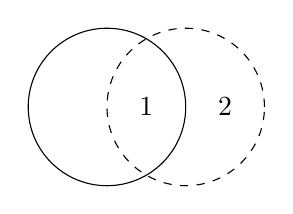
\begin{tikzpicture}
                  \draw (0,0) circle (1cm);
                  \draw[dashed] (1,0) circle (1cm);
                  \node at (0.5,0) {1};
                  \node at (1.5,0) {2};
              \end{tikzpicture}
          \end{figure}

          So, for $n \geq 2$,
          \begin{align*}
              C_n & = C_{n-1} + 2\times(n-1)                                             \\
                  & = C_{n-2} + 2\times(n-2) + 2\times(n-1)                              \\
                  & = C_{1} + 2\times1 + 2\times2 + \ldots + 2\times(n-2) + 2\times(n-1) \\
                  & = 2 + 2\times(1+2+\ldots+(n-2)+(n-1))                                \\
                  & = 2+2\times\frac{n(n-1)}{2}                                          \\
                  & = n^2-n+2                                                            \\
          \end{align*}
          For $n=4$, we get $C_4=14$. We can have at most $14$ regions ($13$ inner, $1$ outer) with $4$ circles intersecting each other.
          \begin{figure}[h!]
              \centering
              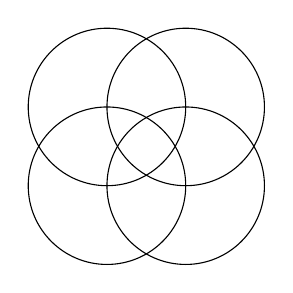
\begin{tikzpicture}
                  \draw (0,0) circle (1cm);
                  \draw (1,0) circle (1cm);
                  \draw (0,1) circle (1cm);
                  \draw (1,1) circle (1cm);
              \end{tikzpicture}
          \end{figure}
\end{itemize}
\clearpage
\section*{Problem 6}
In the original problem, the maximum number of regions, both bounded and unbounded for $n$ line segments was bounded by $O(n^2)$. So, the maximum number of \textit{only bounded} regions must also be bounded by $O(n^2)$.

Let us assume that the solution is $B_n=an^2+bn+c$, where $B_n$ indicates the maximum number of bounded regions possible by $n$ straight lines.
\begin{itemize}
    \item For $n=1$, we have a single line, and no bounded regions, hence $B_1 = 0$.
          \begin{equation}
              a+b+c=0 \tag{1}
          \end{equation}
    \item For $n=2$, we have two intersecting lines, and no bounded regions. Hence $B_2=0$.
          \begin{equation}
              4a+2b+c=0 \tag{2}
          \end{equation}
          \vspace{-.5cm}
          \begin{figure}[h!]
              \centering
              \begin{tikzpicture}
                  \draw (0,0) -- (2,2);
                  \draw (1.3,0) -- (1.3,2);
              \end{tikzpicture}
          \end{figure}
    \item For $n=3$, we have a single bounded region, so $B_3=1$.
          \begin{equation}
              9a+3b+c = 1 \tag{3}
          \end{equation}
          \vspace{-.5cm}
          \begin{figure}[h!]
              \centering
              \begin{tikzpicture}
                  \draw (0,0) -- (2,2);
                  \draw (1.4,0) -- (1.4,2);
                  \draw (0,0.3) -- (2, 0.3);
              \end{tikzpicture}
          \end{figure}
\end{itemize}
Solving these system of equations $(1), (2) \text{ and } (3)$, we get:
\begin{align*}
    a   & =\frac{1}{2}                        \\
    b   & =-\frac{3}{2}                       \\
    c   & =1                                  \\
    B_n & =\frac{n^2}{2} - \frac{3n^2}{2} + 1
\end{align*}
\clearpage

\section*{Problem 10}
We denote the other peg as $C$. For this problem, we can move the disks only clockwise, that is either from $A$ to $B$, $B$ to $C$ or $C$ to $A$. From the problem statement,
\begin{enumerate}[label=(\roman*)]
    \item $Q_n$ is the number of moves required to shift $n$ disks from peg $A$ to peg $B$ under the given restrictions. Since the moves are symmetric, shifting $n$ disks from $B$ to $C$ or $C$ to $A$ require the same number of moves as shifting from $A$ to $B$.
    \item $R_n$ is the number of moves required to shift $n$ disks from $B$ to $A$. By the same reasoning, shifting $n$ disks from $C$ to $B$ or $A$ to $C$ also require $R_n$ number of moves.
\end{enumerate}

\tikzfig{fig10_1} $\implies Q_n =$

\tikzfig{fig10_2} $ R_{n-1}$ (move $n-1$ disks from $A$ to $C$)\\

\tikzfig{fig10_3} $ +1$ (move $n$th disk from $A$ to $B$)\\

\tikzfig{fig10_4} $ +R_{n-1}$ (move $n-1$ disks from $C$ to $B$)

\begin{align}
    Q_n & = R_{n-1} + 1 + R_{n-1} \nonumber \\
        & =2R_{n-1} + 1 \label{eq:10_1}
\end{align}

\tikzfig{fig10_10} $\implies R_n=$\\
\tikzfig{fig10_5} $R_{n-1}$ (move $n-1$ disks from $B$ to $A$)\\
\tikzfig{fig10_6} $+1$ (move $n$th disk from $B$ to $C$)\\
\tikzfig{fig10_7} $+Q_{n-1}$ (move $n-1$ disks from $A$ to $B$)\\
\tikzfig{fig10_8} $+1$ (move $nth$ disk from $C$ to $A$)\\
\tikzfig{fig10_9} $+R_{n-1}$ (move $n-1$ disks from $B$ to $A$)
\begin{align}
    R_n & = R_{n-1} + 1 + Q_{n-1} + 1 + R_{n-1} \nonumber \\
        & =2R_{n-1} + 2 + Q_{n-1} \label{eq:10_2}
\end{align}

From \eqref{eq:10_1}, we can rewrite $2R_{n-1}$ as:
\begin{align}
    2R_{n-1} = Q_n - 1
\end{align}

Replacing this in \eqref{eq:10_2}, we get:
\begin{align}
    R_n & = Q_n - 1 + 2 + Q_{n-1} \nonumber \\
        & = Q_n + Q_{n-1} + 1
\end{align}
Therefore,

\begin{minipage}{.5\textwidth}
    \begin{equation*}
        Q_n =
        \begin{cases}
            0            & \text{if } n=0   \\
            2R_{n-1} + 1 & \text{if } n > 0
        \end{cases}
    \end{equation*}
\end{minipage}%
\begin{minipage}{0.5\textwidth}
    \begin{equation*}
        R_n =
        \begin{cases}
            0                 & \text{if } n=0   \\
            Q_n + Q_{n-1} + 1 & \text{if } n > 0
        \end{cases}
    \end{equation*}
\end{minipage}
\section*{Problem 11}
\begin{enumerate}
    \item Since each of the disks contains an identical copy, we would need exactly 2 moves for moving a single disk including its copy form one peg to another. Hence the total number of moves is just the twice of the original solution, that is $2 \times (2^n-1)$.
          \begin{figure}[h!]
              \centering
              \tikzfig{fig11_1}
              \caption*{Each disk of the same size is indistinguishable from its pair}
              \label{fig:fig11_1}
          \end{figure}
    \item Now the disks contain a copy of the same size, but each of the copies is now \textit{distinguishable} from its pair. The additional constraint now imposed is that we would like to shift the disks in a way so that the original ordering is maintained.
          \begin{figure}[h!]
              \centering
              \tikzfig{fig11_2}
              \label{fig:fig11_2}
          \end{figure}

          We distinguish each pair by giving alternating colors. We can interpret the given constraint in this way:

          ``\textit{The final arrangement should not contain any black disk under a white disk of the same size.}''
\end{enumerate}

This rephrased constraint ensures that the original ordering in the initial arrangement is maintained in the final arrangement. Let us assume that we need $D_{n}$ moves to move such a stack of disks under the given constraints from one peg to another.
\clearpage

\tikzfig{fig11_3} $\implies D_n = $\\
\tikzfig{fig11_4} $D_{n-1} +$\\
\tikzfig{fig11_5} $1 +$\\
\tikzfig{fig11_6} $D_{n-1}+$ \\
\tikzfig{fig11_7} $1+$\\
\tikzfig{fig11_8} $D_{n-1}+$\\
\tikzfig{fig11_9} $1+$\\
\tikzfig{fig11_10} $D_{n-1}$

\begin{align}
    D_n & = D_{n-1} + 1 + D_{n-1} + 1 + D_{n-1} + 1 + D_{n-1} \nonumber \\
        & = 4D_{n-1} + 3
\end{align}

In order to solve this recurrence, we can simplify a bit. We first add $1$ to both sides, giving:
\begin{align*}
    D_n + 1 & = 4D_{n-1} + 4  \\
            & =4(D_{n-1} + 1)
\end{align*}
If we let $Z_n = D_n + 1$, we get:
\begin{align*}
    Z_n & = 4Z_{n-1}
\end{align*}
Since $D_0=0$, $Z_0 = D_0 + 1 = 1$, we can simply unwind the recurrence and find the solution to $Z_n$ directly:
\begin{align*}
    Z_n          & = 4^n   \\
    \implies D_n & = 4^n-1
\end{align*}
\clearpage

\section*{Problem 13}
Let $ZZ_n$ denote the maximum number of regions defined by $n$ zig-zag lines. Here,
\begin{align*}
    ZZ_0 & = 1 \\
    ZZ_1 & = 2
\end{align*}
To find a recurrence relation, we notice the following:
\begin{enumerate}[label=(\roman*)]
    \item Assume we are dealing with straight lines only, no zig-zags. When the $n$th line intersects the previous $n-1$ lines into $n-1$ distinct points, it creates $n$ additional regions.
    \item Now assume that we make zig-zags out of each line in the following way:
          \begin{center}
              \tikzfig{fig13_5} $\implies$ \tikzfig{fig13_3} $\implies$ \tikzfig{fig13_4}
          \end{center}

          In this way, if we make the $n$th line a zig-zag, for each of the previous $n-1$ zig-zags, it will introduce $8$ \textit{new} bounded regions.
          \begin{center}
              \tikzfig{fig13_1} $\implies$ \tikzfig{fig13_2}
          \end{center}
          We will get $8\times (n-1)$ new bounded regions in this way.
\end{enumerate}
Thus, from (i) we get $n$ regions, and from (ii) we get $8\times (n-1)$ new bounded regions. We can define $ZZ_n$ as:
\begin{align}
    ZZ_n & = ZZ_{n-1} + 8\times(n-1) + n \nonumber \\
         & = ZZ_{n-1} + 9n - 8
\end{align}
We can solve this recurrence using perturbation method, or we can break it down into a simpler one:
\begin{align}
    ZZ_n - n & = ZZ_{n-1} - (n-1) + 9(n-1) \label{eq:13_1}
\end{align}
Equation \eqref{eq:13_1} was obtained from observation in such a way so that we can let $T_n = ZZ_n - n$. The base cases are:
\begin{align*}
    T_0 & = 1 - 0 = 1 \\
    T_1 & = 2 - 1 = 1
\end{align*}
Replacing $T_n = ZZ_n - n$ in \eqref{eq:13_1}:
\begin{align*}
    T_n               & = T_{n-1} + 9(n-1)                                     \\
                      & = T_{n-2} + 9(n-2) + 9(n-1)                            \\
                      & = T_1 + 9\times1 + 9\times2 + \ldots + 9(n-2) + 9(n-1) \\
                      & = 1 + 9\times(1+2+\ldots+(n-2) + (n-1))                \\
                      & = 1 + 9\times \frac{n(n-1)}{2}                         \\
    \implies ZZ_n - n & = 1 + \frac{9n^2-9n}{2}                                \\
    \implies ZZ_n     & = \frac{9n^2}{2} - \frac{7n}{2} + 1
\end{align*}

\section*{Problem 14}
Let us look at a few base cases first. We would use the word \textit{region} to indicate a 2-dimensional slice, and the word \textit{space} to indicate a 3-dimensional slice. When there are no planes through the cube, we get only $1$ space, the whole cube itself.
\begin{figure}[h!]
    \centering
    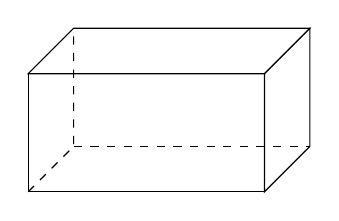
\begin{tikzpicture}
\pgfmathsetmacro{\cubex}{3}
\pgfmathsetmacro{\cubey}{1.5}
\pgfmathsetmacro{\cubez}{1.5}
\draw[black] (0,0,0) -- ++(-\cubex,0,0) -- ++(0,-\cubey,0) -- ++(\cubex,0,0) -- cycle;
\draw[black] (0,0,0) -- ++(0,0,-\cubez) -- ++(0,-\cubey,0) -- ++(0,0,\cubez) -- cycle;
\draw[black] (0,0,0) -- ++(-\cubex,0,0) -- ++(0,0,-\cubez) -- ++(\cubex,0,0) -- cycle;
\draw[black, dashed] (-\cubex, -\cubey, -\cubez) -- ++(\cubex, 0, 0);
\draw[black, dashed] (-\cubex, -\cubey, 0) -- ++(0,0,-\cubez) -- ++(0,\cubey,0);
\end{tikzpicture}
\end{figure}

Adding a single plane splits the cube into $2$ distinct spaces.
\begin{figure}[h!]
    \centering
    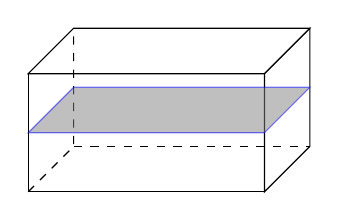
\begin{tikzpicture}
\pgfmathsetmacro{\cubex}{3}
\pgfmathsetmacro{\cubey}{1.5}
\pgfmathsetmacro{\cubez}{1.5}
\draw[black] (0,0,0) -- ++(-\cubex,0,0) -- ++(0,-\cubey,0) -- ++(\cubex,0,0) -- cycle;
\draw[black] (0,0,0) -- ++(0,0,-\cubez) -- ++(0,-\cubey,0) -- ++(0,0,\cubez) -- cycle;
\draw[black] (0,0,0) -- ++(-\cubex,0,0) -- ++(0,0,-\cubez) -- ++(\cubex,0,0) -- cycle;
\draw[black, dashed] (-\cubex, -\cubey, -\cubez) -- ++(\cubex, 0, 0);
\draw[black, dashed] (-\cubex, -\cubey, 0) -- ++(0,0,-\cubez) -- ++(0,\cubey,0);
\draw[blue,fill=gray,opacity=0.5] (-\cubex,-\cubey/2,0) -- ++(\cubex,0,0) -- ++(0,0,-\cubez) -- ++(-\cubex,0,0) -- cycle;
\end{tikzpicture}
\end{figure}

It is clear that we get $4$ separate spaces when there are $2$ planes. One may think it like this: the new vertical plane is divided into $2$ distinct regions by the previous horizontal plane. Their intersection is indicated by a solid line. For each of the divided region in the vertical plane, a single new space is introduced in addition to the previous one, thus we get $2 + 2 = 4$ total spaces.
\begin{figure}[h!]
    \centering
    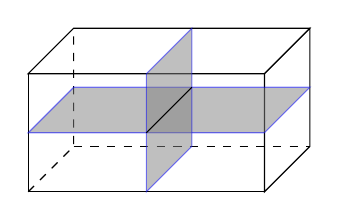
\begin{tikzpicture}
\pgfmathsetmacro{\cubex}{3}
\pgfmathsetmacro{\cubey}{1.5}
\pgfmathsetmacro{\cubez}{1.5}
\draw[black] (0,0,0) -- ++(-\cubex,0,0) -- ++(0,-\cubey,0) -- ++(\cubex,0,0) -- cycle;
\draw[black] (0,0,0) -- ++(0,0,-\cubez) -- ++(0,-\cubey,0) -- ++(0,0,\cubez) -- cycle;
\draw[black] (0,0,0) -- ++(-\cubex,0,0) -- ++(0,0,-\cubez) -- ++(\cubex,0,0) -- cycle;
\draw[black, dashed] (-\cubex, -\cubey, -\cubez) -- ++(\cubex, 0, 0);
\draw[black, dashed] (-\cubex, -\cubey, 0) -- ++(0,0,-\cubez) -- ++(0,\cubey,0);
\draw[blue,fill=gray,opacity=0.5] (-\cubex,-\cubey/2,0) -- ++(\cubex,0,0) -- ++(0,0,-\cubez) -- ++(-\cubex,0,0) -- cycle;
\draw[blue,fill=gray,opacity=0.5] (-\cubex/2,0,0) -- ++(0,-\cubey,0) -- ++(0,0,-\cubez) -- ++(0,\cubey,0) -- cycle;
\draw[black] (-\cubex/2, -\cubey/2, 0) -- ++(0,0,-\cubez);
\end{tikzpicture}
\end{figure}
\clearpage

Adding the $3$rd plane divides the cube into $8$ separate spaces. The $3$rd planes intersects with the previous $2$ planes, which gives $2$ intersection lines (indicated by the dotted black lines). These $2$ dotted lines divide the $3$rd plane into $4$ separate regions. For each of these regions, we get a new space in addition to the previous $4$, thus we get $4 + 4 = 8$ total spaces.
\begin{figure}[h!]
    \centering
    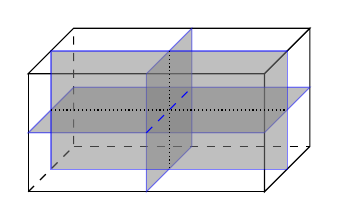
\begin{tikzpicture}
\pgfmathsetmacro{\cubex}{3}
\pgfmathsetmacro{\cubey}{1.5}
\pgfmathsetmacro{\cubez}{1.5}
\draw[black] (0,0,0) -- ++(-\cubex,0,0) -- ++(0,-\cubey,0) -- ++(\cubex,0,0) -- cycle;
\draw[black] (0,0,0) -- ++(0,0,-\cubez) -- ++(0,-\cubey,0) -- ++(0,0,\cubez) -- cycle;
\draw[black] (0,0,0) -- ++(-\cubex,0,0) -- ++(0,0,-\cubez) -- ++(\cubex,0,0) -- cycle;
\draw[black, dashed] (-\cubex, -\cubey, -\cubez) -- ++(\cubex, 0, 0);
\draw[black, dashed] (-\cubex, -\cubey, 0) -- ++(0,0,-\cubez) -- ++(0,\cubey,0);
\draw[blue,fill=gray,opacity=0.5] (-\cubex,-\cubey/2,0) -- ++(\cubex,0,0) -- ++(0,0,-\cubez) -- ++(-\cubex,0,0) -- cycle;
\draw[blue,fill=gray,opacity=0.5] (-\cubex/2,0,0) -- ++(0,-\cubey,0) -- ++(0,0,-\cubez) -- ++(0,\cubey,0) -- cycle;
\draw[blue,fill=gray,opacity=0.5] (-\cubex,0,-\cubez/2) -- ++(\cubex,0,0) -- ++(0,-\cubey,0) -- ++(-\cubex,0,0) -- cycle;
\draw[blue, dashed] (-\cubex/2, -\cubey/2, 0) -- ++(0,0,-\cubez);
\draw[black, densely dotted] (-\cubex/2, 0, -\cubez/2) -- ++(0,-\cubey,0);
\draw[black, densely dotted] (-\cubex, -\cubey/2, -\cubez/2) -- ++(\cubex,0,0);
\end{tikzpicture}
\end{figure}

\begin{figure}[h!]
    \centering
    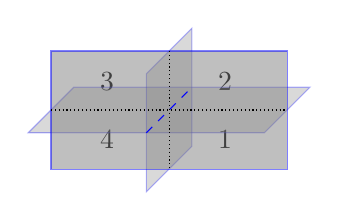
\begin{tikzpicture}
\pgfmathsetmacro{\cubex}{3}
\pgfmathsetmacro{\cubey}{1.5}
\pgfmathsetmacro{\cubez}{1.5}
\node at (-\cubex/6, -\cubey/1.8) {1};
\node at (-\cubex/6, -.1) {2};
\node at (-2, -.1) {3};
\node at (-2, -\cubey/1.8) {4};
\draw[blue,fill=gray,opacity=0.3] (-\cubex,-\cubey/2,0) -- ++(\cubex,0,0) -- ++(0,0,-\cubez) -- ++(-\cubex,0,0) -- cycle;
\draw[blue,fill=gray,opacity=0.3] (-\cubex/2,0,0) -- ++(0,-\cubey,0) -- ++(0,0,-\cubez) -- ++(0,\cubey,0) -- cycle;
\draw[blue,fill=gray,opacity=0.5] (-\cubex,0,-\cubez/2) -- ++(\cubex,0,0) -- ++(0,-\cubey,0) -- ++(-\cubex,0,0) -- cycle;
\draw[blue, dashed] (-\cubex/2, -\cubey/2, 0) -- ++(0,0,-\cubez);
\draw[black, densely dotted] (-\cubex/2, 0, -\cubez/2) -- ++(0,-\cubey,0);
\draw[black, densely dotted] (-\cubex, -\cubey/2, -\cubez/2) -- ++(\cubex,0,0);
\end{tikzpicture}
\end{figure}

We can see a pattern forming from the base cases. The $n$th plane is intersected by the previous $n-1$ planes, which can be though of as $n-1$ intersection lines through the $n$th plane. We know that the number of regions formed by $n-1$ lines through a plane is $L_{n-1}$. For each of these regions, we are getting a new space. So the number of new spaces is the same as $L_{n-1}$.\\

If we denote $P_n$ as the maximum number of $3$-dimensional spaces that can be defined by $n$ planes, we can define $P_n$ as:
\begin{align}
    P_n = P_{n-1} + L_{n-1}
\end{align}

\section*{Problem 15}
The problem is undefined for $n=1$, we will assume $n\geq2$. We can split the problem into two cases:
\begin{enumerate}[label=(\roman*)]
    \item Even number of people: If we start with $2n$ persons, after the first round all the even numbered persons will be eliminated. Just like the original problem, we can write:
          $$I(2n) = 2I(n) - 1$$
    \item Odd number of people: Similarly for this case, we can write:
          $$I(2n + 1) = 2I(n) + 1$$
\end{enumerate}
\begin{table}[h!]
    \centering
    \begin{tabular}{L|LLLLLLLLLLLL}
        n    & 1      & 2 & 3 & 4 & 5 & 6 & 7 & 8 & 9 & 10 & 11 & 12 \\ \hline
        I(n) & \times & 2 & 1 & 3 & 5 & 1 & 3 & 5 & 7 & 9  & 11 & 1
    \end{tabular}
    \caption*{First few values for the penultimate number}
    \label{tab:tab_15}
\end{table}
\clearpage
If we look at the values of $n$ for which $I(n) = 1$, we get $n = 3,6,12,\ldots = 3\times 2^0, 3\times2^1, 3\times2^2, \ldots$.

If we write $n = 3\times2^m + r$, where $m$ is the highest integer such that $3\times2^m\leq n$, then we can propose $I(n)= I(3\times2^m + r) = 2r + 1$. This formula checks out for other values as well, for example: $n=8=3\times2^2 + 2$, $I(8) = 2\times2 + 1 = 5$. This is our proposed hypothesis. We can use proof by induction to check if this is indeed correct.\\

\textit{Base case}: $n=2=3\times2^{-1} + \frac{1}{2} \implies I(\frac{1}{2})= 2\times \frac{1}{2} + 1 = 2$ \\

\textit{Inductive hypothesis:} Assume the formula holds for $m=2,3,\ldots,k$

$I(n)=I(3\times 2^k + r) = 2r+1$\\

\textit{Proof:} We have to show that the formula holds for $m=k+1$.

\begin{enumerate}[label=(\roman*)]
    \item $n = 3\times2^k + r$ even:
          \begin{align*}
                       & I(3\times 2^{(k+1)} + r)                                             \\
              \implies & I(3\times2^k\times2 + r)                                             \\
              \implies & 2I(3\times2^k + \frac{r}{2}) - 1 \qquad \text{Since $I(2n)=2I(n)-1$} \\
              \implies & 2(2\times\frac{r}{2} + 1) - 1                                        \\
              \implies & 2r + 1
          \end{align*}
    \item $n = 3\times2^k + r$ odd:
          \begin{align*}
                       & I(3\times 2^{(k+1)} + r)                                                 \\
              \implies & I(3\times2^k\times2 + (r-1)+1)                                           \\
              \implies & 2I(3\times2^k + \frac{r-1}{2}) + 1 \qquad \text{Since $I(2n+1)=2I(n)+1$} \\
              \implies & 2(2\times\frac{r-1}{2} + 1) + 1                                          \\
              \implies & 2r + 1
          \end{align*}
\end{enumerate}

Thus $I(n) = I(3\times2^m + r) = 2r + 1$ is the required formula for $n\geq2$.
\clearpage
\section*{Problem 17}
If we place the head of a zig inside another zig, we won't be able to achieve the maximum number of regions, $Z_n$. From the figure below, we can see that there are only $2$ intersection points and we have a total of $5$ regions.
\ctikzfig{fig17_1}

In order to maximize the number of regions, we would need to maximize the number of intersections as well. For that we have to place the head of each zigs outside the region of another one. In the figure below, we obtain $4$ intersection points and $7$ regions, which is the maximum possible number. The mapping from intersection points to the number of regions is distinct: We have $7$ regions if and only if we have $4$ intersection points. This holds for other values as well when the number of regions is maximized.
\ctikzfig{fig17_3}


Now let us think about a modified version of the problem. Suppose that each zigs has an angle of $90^{\circ}$. We know from the previous example that we can have at most $7$ regions with $2$ zigs, and those zigs must intersect at $4$ distinct points. When each of the two zigs is at $90^{\circ}$, no matter how hard we try, it is impossible to get more than $3$ intersection points, which gives a maximum of $6$ regions. There will always be at least one line for each zig that will keep diverging from another line of the other zig.
\begin{figure}[h!]
    \centering
    \tikzfig{fig17_2}
    \caption*{The dashed lines do not intersect and diverge from each other}
    \label{fig17_2}
\end{figure}

The reasoning is simple: two $90^{\circ}$s add up to $180^{\circ}$, in order to have $4$ intersection points, at least one of the zigs need to have an angle  $<90^{\circ}$. We can go the other way around: when the angle of each zigs is at $90^{\circ}$, we will have $< (\frac{180}{90} = 2)$ zigs that will give the maximum number of regions. For problem 17, the angle is $30^{\circ}$ and we will have $< (\frac{180}{30} = 6)$ zigs that can obtain $Z_n$ number of regions. The maximum integer $<6$ is $5$.

\pagebreak
\begin{center}
    {\huge Chapter 2}
\end{center}
\section*{Problem 11}
\begin{align*}
      & \sum_{0\leq k < n} (a_{k+1}-a_k)b_k                                                     \\
    = & \sum_{0\leq k < n} (a_{k+1}b_k - a_k b_k)                                               \\
    = & \sum_{0\leq k < n} a_{k+1}b_k -\sum_{0\leq k < n} a_k b_k                               \\
    = & \sum_{0\leq k < n} a_{k+1}b_k - \sum_{1\leq k < n + 1} a_kb_k - (a_0b_0-a_nb_n)         \\
    = & \sum_{0\leq k < n} a_{k+1}b_k - \sum_{1\leq k+1 < n + 1} a_{k+1}b_{k+1} + a_nb_n-a_0b_0 \\
    = & \sum_{0\leq k < n} a_{k+1}b_k - \sum_{0\leq k < n} a_{k+1}b_{k+1} + a_nb_n-a_0b_0       \\
    = & \sum_{0\leq k < n} (a_{k+1}b_k - a_{k+1}b_{k+1}) + a_nb_n-a_0b_0                        \\
    = & \;a_nb_n-a_0b_0 - \sum_{0 \leq k < n} {a_{k+1}(b_{k+1}-b_k)}
\end{align*}
\section*{Problem 12}
If we can find an inverse function of $p(k)$ whose domain is defined for the set of all integers, then the range of $p(k)$ will contain the set of all integers. Let,
\begin{align*}
    p(k)     & = k + (-1)^kc = y \stampeq \label{eq:12_1}     \\
    \implies & = y+c = k+ \underbrace{\left(1+(-1)^k\right)}c \\
\end{align*}
Here,\[
    \left(1+(-1)^k\right) = \begin{dcases*}
        0 & $k$ odd  \\
        2 & $k$ even
    \end{dcases*}
\]
So, $y+c$ and $k$ have the same parity: they are either both even or both odd. So we can write: $(-1)^{y+c} = (-1)^k$. From \eqref{eq:12_1}:
\begin{align*}
    y          & = k + (-1)^k c    \\
    \implies y & = k + (-1)^{y+c}c \\
    \implies k & = y-(-1)^{y+c}c
\end{align*}
Therefore, $q(y) = y-(-1)^{y+c}c$ is defined for the set of all integers. Hence the range of $p(k)$ contains the set of all integers.
\section*{Problem 14}
\begin{align*}
    S_n & = \sum_{k=1}^{n} k2^k                  \\
        & = \sum_{k=1}^n \sum_{j=1}^k 1\times2^k \\
        & =\sum_{j=1}^n \sum_{k=j}^n 2^k         \\
        & =\sum_{j=1}^n 2^{n+1}-2^j              \\
        & =n2^{n+1}-\sum_{j=1}^n 2^j             \\
        & =n2^{n+1}-(2^{n+1}-2)
\end{align*}
\section*{Problem 19}
Here,
\begin{align*}
    a  2                                                                               \\ b_n &= n\\ c_n &= 3\cdot n!\\
    \therefore s_n & = \frac{a_{n-1}a_{n-2}\ldots a_1}{b_nb_{n-1}\ldots b_2}\times s_1 \\
                   & =\frac{2^{n-1}}{n!} \qquad \text{[Letting $s_1=1$]}
\end{align*}
Now,
\begin{align*}
             & s_na_nT_n = s_1b_1T_0 + \sum_{k=1}^{n} s_kc_k                                         \\
    \implies & \frac{2^{n-1}}{n!}\cdot 2\cdot T_n= 5+\sum_{k=1}^n \frac{2^{k-1}}{k!}\times 3\cdot k! \\
    \implies & \frac{2^n}{n!}T_n = 5 + 3\sum_{k=1}^n{2^{k-1}}                                        \\
    \implies & \frac{2^n}{n!}T_n = 5 + 3 \times (2^n - 1)                                            \\
    \implies & T_n = \frac{n!}{2^n} (2 + 3\times 2^n)                                                \\
    \implies & T_n = \frac{n!}{2^{n-1}} + 3n!
\end{align*}

\section*{Problem 20}
\begin{align*}
     & S_n = \sum_{k=0}^n kH_k \\
\end{align*}
Here,
\begin{align*}
    S_{n+1} & = \sum_{k=0}^{n+1} kH_k                      \\
            & = \sum_{k=0}^n kH_k + (n+1)H_{n+1}           \\
            & =S_n + (n+1)H_{n+1} \stampeq \label{eq:20_1}
\end{align*}
Again,
\begin{align*}
    S_{n+1} & = \sum_{k=0}^{n+1} kH_k                                  \\
            & =\sum_{1\leq k \leq n+1} kH_k + 0\times H_0              \\
            & =\sum_{1\leq k+1 \leq n+1} (k+1)H_{k+1}                  \\
            & =\sum_{0\leq k \leq n} (k+1)(H_k + \frac{1}{k+1})        \\
            & =\sum_{k=0}^n kH_k + H_k + 1                             \\
            & =S_n + \sum_{k=0}^n H_k + (n+1) \stampeq \label{eq:20_2}
\end{align*}

From \eqref{eq:20_1} and \eqref{eq:20_2},
\begin{align*}
             & S_n + (n+1)H_{n+1} = S_n + \sum_{k=0}^n H_k + (n+1) \\
    \implies & \sum_{k=0}^n H_k = (n+1)(H_{n+1}-1)
\end{align*}
\clearpage
\section*{Problem 21}
\[
    S_n = \sum_{0\leq k \leq n} (-1)^{n-k}\\
\]
\begin{align*}
    S_{n+1} & =\sum_{0\leq k \leq n+1} (-1)^{n-k}                 \\
            & = (-1)^{n-(n+1)} + \sum_{0\leq k \leq n} (-1)^{n-k} \\
            & = -1 + S_n \stampeq \label{eq:21_1}
\end{align*}
\begin{align*}
    S_{n+1} & =\sum_{0\leq k \leq n+1} (-1)^{n-k}              \\
            & =(-1)^{n-0} + \sum_{1\leq k \leq n+1} (-1)^{n-k} \\
            & =(-1)^n + \sum_{0\leq k \leq n} (-1)^{n-(k+1)}   \\
            & =(-1)^n -\sum_{0_\leq k \leq n}(-1)^{n-k}        \\
            & =(-1)^n - S_n \stampeq \label{eq:21_2}
\end{align*}
From \eqref{eq:21_1} and \eqref{eq:21_2},
\begin{align*}
    -1 + S_n     & = (-1)^n -S_n                                 \\
    \implies S_n & = \frac{1+(-1)^n}{2} \stampeq \label{eq:21_3}
\end{align*}
Again,
\[
    T_n = \sum_{0 \leq k \leq n} (-1)^{n-k}k
\]
\begin{align*}
    T_{n+1} & = \sum_{0 \leq k \leq n+1} (-1)^{n-k}k                    \\
            & =(-1)^{n-(n+1)}(n+1) + \sum_{0 \leq k \leq n} (-1)^{n-k}k \\
            & =-(n+1) + T_n \stampeq \label{eq:21_4}
\end{align*}
\begin{align*}
    T_{n+1} & = \sum_{0 \leq k \leq n+1} (-1)^{n-k}k                                \\
            & =(-1)^{n-0}\times 0 + \sum_{1 \leq k \leq n+1}(-1)^{n-k}k             \\
            & =0 + \sum_{0 \leq k \leq n} (-1)^{n-(k+1)}(k+1)                       \\
            & =-\sum_{0\leq k \leq n} (-1)^{n-k}(k+1)                               \\
            & =-\sum_{0\leq k \leq n} (-1)^{n-k}k - \sum_{0\leq k \leq n}(-1)^{n-k} \\
            & =-T_n-S_n \stampeq \label{eq:21_5}
\end{align*}
From \eqref{eq:21_4} and \eqref{eq:21_5},
\begin{align*}
    -(n+1) + T_n & = -T_n-S_n                                   \\
    \implies T_n & = \frac{1+n-S_n}{2} \stampeq \label{eq:21_6}
\end{align*}
Finally,
\[
    U_n = \sum_{0 \leq k \leq n} (-1)^{n-k}k^2
\]
\begin{align*}
    U_{n+1} & = \sum_{0 \leq k \leq n+1} (-1)^{n-k}k^2         \\
            & = -(n+1)^2 + \sum_{0 \leq k \leq n}(-1)^{n-k}k^2 \\
            & = -(n+1)^2 + U_n \stampeq \label{eq21:7}
\end{align*}
\begin{align*}
    U_{n+1} & = \sum_{0 \leq k \leq n+1} (-1)^{n-k}k^2                                                                     \\
            & = 0 + \sum_{1 \leq k \leq n+1}(-1)^{n-k}k^2                                                                  \\
            & = \sum_{0 \leq k \leq n}(-1)^{n-(k+1)}(k+1)^2                                                                \\
            & = -\sum_{0 \leq k \leq n}(-1)^{n-k}(k^2 + 2k + 1)                                                            \\
            & = -\sum_{0 \leq k \leq n}(-1)^{n-k}k^2 -2\sum_{0 \leq k \leq n}(-1)^{n-k}k -\sum_{0 \leq k \leq n}(-1)^{n-k} \\
            & = -U_n - 2T_n - S_n \stampeq \label{eq:21_8}
\end{align*}

From \eqref{eq21:7} and \eqref{eq:21_8},
\begin{align*}
    -(n+1)^2 & + U_n = -U_n - 2T_n - S_n                                    \\
    \implies & U_n = \frac{(n+1)^2 - 2T_n -S_n}{2} \stampeq \label{eq:21_9}
\end{align*}

\section*{Problem 22}
Proof of \textit{Lagrange's Identity:}
\[
    \sum_{1\leq j < k \leq n} (a_jb_k-a_kb_j)^2 = \left(\sum_{k=1}^n {a_k}^2\right) \left(\sum_{k=1}^n {b_k}^2\right) - \left(\sum_{k=1}^n {a_kb_k}^2\right)
\]
Let,
\begin{align*}
    S             & = \sum_{1\leq j < k \leq n} (a_jb_k-a_kb_j)^2 \quad \scalebox{0.2}{\tikzfig{triup}}                                                 \\
    S             & = \sum_{1\leq k < j \leq n} (a_kb_j-a_jb_k)^2 \quad \scalebox{0.2}{\tikzfig{trilow}} \qquad \text{[Swapping $j \leftrightarrow k$]} \\
    \therefore 2S & = \sum_{1\leq j,k \leq n} (a_kb_j-a_jb_k)^2 - \sum_{1\leq j=k \leq n} (a_kb_j-a_jb_k)^2 \quad \scalebox{0.2}{\tikzfig{triboth}}     \\
                  & = \sum_{1\leq j,k \leq n} (a_kb_j-a_jb_k)^2 -0                                                                                      \\
                  & = \sum_{j} \sum_{k}(a_k^2b_j^2 - 2a_ja_kb_jb_k + a_j^2b_k^2)[1\leq j \leq n][1\leq k \leq n]                                        \\
    \begin{split}
        &=\sum_{j}b_j^2[1\leq j \leq n]\sum_{k}a_k^2[1\leq k \leq n]-2\sum_{j}a_jb_j[1\leq j \leq n]\sum_{k}a_kb_k[1\leq k \leq n] \\
        &+ \sum_{j}a_j^2[1\leq j \leq n]\sum_{k}b_k^2[1\leq k \leq n]
    \end{split}                          \\
    \begin{split}
        &=\sum_{k}b_k^2[1\leq k \leq n]\sum_{k}a_k^2[1\leq k \leq n]-2\sum_{k}a_kb_k[1\leq k \leq n]\sum_{k}a_kb_k[1\leq k \leq n] \\
        &+ \sum_{k}a_k^2[1\leq k \leq n]\sum_{k}b_k^2[1\leq k \leq n]
    \end{split}
\end{align*}
\begin{align*}
             & =\sum_{1\leq k \leq n}b_k^2\sum_{1\leq k \leq n}a_k^2-2\sum_{1\leq k \leq n}a_kb_k\sum_{1\leq k \leq n}a_kb_k + \sum_{1\leq k \leq n}a_k^2\sum_{1\leq k \leq n}b_k^2 \\
             & =2\left(\sum_{1\leq k \leq n}a_k^2\right)\left(\sum_{1\leq k \leq n}b_k^2\right)-2\left(\sum_{1\leq k \leq n}a_kb_k\right)^2                                         \\
    \implies & S = \left(\sum_{1\leq k \leq n}a_k^2\right)\left(\sum_{1\leq k \leq n}b_k^2\right)-\left(\sum_{1\leq k \leq n}a_kb_k\right)^2
\end{align*}
With a similar approach, we can prove:
\begin{align*}
    \sum_{1\leq j < k \leq n} (a_jb_k-a_kb_j)(A_jB_k-A_kB_j) = \left(\sum_{1\leq k \leq n}a_kA_k\right)\left(\sum_{1\leq k \leq n}b_kB_k\right)-\left(\sum_{1\leq k \leq n}a_kB_k\right)\left(\sum_{1\leq k \leq n}A_kb_k\right)
\end{align*}

\section*{Problem 23}
\begin{align*}
    S & = \sum_{k=1}^{n} \frac{2k+1}{k(k+1)}                                                      \\
      & =\sum_{k=1}^{n} \left(\frac{1}{k} + \frac{1}{k+1}\right)                                  \\
      & = \sum_{k=1}^{n} \frac{1}{k} + \sum_{k=1}^{n} \frac{1}{k+1}                               \\
      & = H_n + \sum_{1\leq k-1 \leq n} \frac{1}{(k-1)+1} \quad \text{Replace $k\rightarrow k-1$} \\
      & = H_n + \sum_{2\leq k \leq n+1} \frac{1}{k}                                               \\
      & = H_n + \sum_{1\leq k \leq n} \frac{1}{k} - 1 + \frac{1}{n+1}                             \\
      & = 2H_n - 1 + \frac{1}{n+1}
\end{align*}
\section*{Problem 24}
\begin{align*}
    S & = \sum_{0 \leq k < n} \frac{H_k}{(k+1)(k+2)}                                                                                                                                                                                                                                                                      \\
      & = \sum_{0 \leq k \leq n-1} H_k\left(\frac{1}{k+1}-\frac{1}{k+2}\right)                                                                                                                                                                                                                                            \\
      & = 0\cdot\left(\frac{1}{1} - \frac{1}{2}\right) + \left(\frac{1}{1}\right)\cdot\left(\frac{1}{2} - \frac{1}{3}\right) + \left(\frac{1}{1} + \frac{1}{2}\right)\cdot\left(\frac{1}{3} - \frac{1}{4}\right)+\left(\frac{1}{1} + \frac{1}{2} + \frac{1}{3}\right)\cdot\left(\frac{1}{4} - \frac{1}{5}\right) + \ldots \\
    \begin{split}
        &= \frac{1}{1}\left(\frac{1}{2} - \frac{1}{3} + \frac{1}{3} - \frac{1}{4} + \frac{1}{4} - \frac{1}{5} + \ldots + \frac{1}{n}-\frac{1}{n+1}\right)\\
        &+\frac{1}{2}\left(\frac{1}{3} - \frac{1}{4} + \frac{1}{4} - \frac{1}{5} + \ldots + \frac{1}{n}-\frac{1}{n+1}\right)\\
        &+\frac{1}{3}\left(\frac{1}{4} - \frac{1}{5} + \ldots + \frac{1}{n}-\frac{1}{n+1}\right)\\
        &+\cdots\\
        &+\frac{1}{n-1}\left(\frac{1}{n}-\frac{1}{n+1}\right)
    \end{split}                                                                                                                                                                      \\
      & = \frac{1}{1}\left(\frac{1}{2}-\frac{1}{n+1}\right)
    +\frac{1}{2}\left(\frac{1}{3}-\frac{1}{n+1}\right)
    +\frac{1}{3}\left(\frac{1}{4} -\frac{1}{n+1}\right)
    +\cdots +\frac{1}{n-1}\left(\frac{1}{n}-\frac{1}{n+1}\right)                                                                                                                                                                                                                                                          \\
      & = \left(\frac{1}{1\cdot 2}+ \frac{1}{2\cdot 3}+ \frac{1}{3\cdot 4} + \ldots + \frac{1}{(n-1)\cdot n}\right) - \frac{1}{n+1}\left(\frac{1}{1} + \frac{1}{2} + \frac{1}{3} + \cdots + \frac{1}{n-1}\right)                                                                                                          \\
      & =\sum_{1 \leq k \leq n-1} \frac{1}{k(k+1)}  - \frac{1}{n+1} \left(H_n-\frac{1}{n}\right)                                                                                                                                                                                                                          \\
      & =\sum_{1 \leq k \leq n-1} \left(\frac{1}{k}-\frac{1}{k+1}\right)  - \frac{1}{n+1} \left(H_n-\frac{1}{n}\right)                                                                                                                                                                                                    \\
      & =\left(\sum_{1 \leq k \leq n}\frac{1}{k} - \frac{1}{n}\right) - \left(\sum_{1 \leq k-1 \leq n-1}\frac{1}{(k-1)+1}\right) - \frac{1}{n+1} \left(H_n-\frac{1}{n}\right)                                                                                                                                             \\
      & =\left(H_n - \frac{1}{n}\right) - \left(\sum_{2 \leq k \leq n}\frac{1}{k}\right)- \frac{1}{n+1} \left(H_n-\frac{1}{n}\right)                                                                                                                                                                                      \\
      & =\left(H_n - \frac{1}{n}\right) - \left(\sum_{1 \leq k \leq n}\frac{1}{k}-1\right)- \frac{1}{n+1} \left(H_n-\frac{1}{n}\right)                                                                                                                                                                                    \\
      & =\left(H_n - \frac{1}{n} -H_n + 1\right)- \frac{1}{n+1} \left(H_n-\frac{1}{n}\right)                                                                                                                                                                                                                              \\
      & =1-\frac{1}{n}+\frac{1}{n(n+1)}-\frac{H_n}{n+1}                                                                                                                                                                                                                                                                   \\
      & =1-\frac{1}{n+1}-\frac{H_n}{n+1}                                                                                                                                                                                                                                                                                  \\
      & =1-\frac{H_n+1}{n+1}
\end{align*}
\section*{Bonus Problem}
This stemmed from a failed attempt to Problem 24.
\begin{align*}
    S & = 0\cdot\left(\frac{1}{1} - \frac{1}{2}\right) + \frac{1}{1}\cdot\left(\frac{1}{2} - \frac{1}{3}\right) + \frac{1}{2}\cdot\left(\frac{1}{3} - \frac{1}{4}\right)+\frac{1}{3}\cdot\left(\frac{1}{4} - \frac{1}{5}\right) + \ldots \\
      & = 0 + \frac{1}{1\cdot 2} - \frac{1}{1\cdot 3} + \frac{1}{2\cdot 3} - \frac{1}{2\cdot 4} + \frac{1}{3\cdot 4} - \frac{1}{3\cdot 5} + \ldots                                                                                       \\
      & = \left(\frac{1}{1\cdot 2}+ \frac{1}{2\cdot 3}+ \frac{1}{3\cdot 4} + \ldots\right) - \left(\frac{1}{1\cdot 3} +\frac{1}{2\cdot 4} +\frac{1}{3\cdot 5} + \ldots \right)                                                           \\
      & =\sum_{1 \leq k < n} \frac{1}{k(k+1)} - \sum_{1 \leq k < n} \frac{1}{k(k+2)}                                                                                                                                                     \\
      & =\sum_{1 \leq k < n}\frac{1}{k(k+1)(k+2)}                                                                                                                                                                                        \\
      & =\sum_{1 \leq k < n}\left(\frac{1}{2k}-\frac{1}{k+1} + \frac{1}{2(k+2)}\right)                                                                                                                                                   \\
      & =\frac{1}{2}\left(\sum_{1 \leq k \leq n}\frac{1}{k} - \frac{1}{n}\right) - \left(\sum_{1 \leq k-1 < n}\frac{1}{(k-1)+1}\right) + \frac{1}{2}\left(\sum_{1 \leq k-2 < n}\frac{1}{(k-2)+2}\right)                                  \\
      & =\frac{1}{2}\left(H_n - \frac{1}{n}\right) - \left(\sum_{2 \leq k \leq n}\frac{1}{k}\right) + \frac{1}{2}\left(\sum_{3 \leq k \leq n+1}\frac{1}{k}\right)                                                                        \\
      & =\frac{1}{2}\left(H_n - \frac{1}{n}\right) - \left(\sum_{1 \leq k \leq n}\frac{1}{k}-1\right) + \frac{1}{2}\left(\sum_{1 \leq k \leq n}\frac{1}{k} + \frac{1}{n+1} - 1 - \frac{1}{2}\right)                                      \\
      & =\frac{1}{2}\left(H_n - \frac{1}{n}\right) - \left(H_n-1\right) + \frac{1}{2}\left(H_n + \frac{1}{n+1} - 1 - \frac{1}{2}\right)                                                                                                  \\
      & =1-\frac{1}{2n} + \frac{1}{2(n+1)} - \frac{3}{4}                                                                                                                                                                                 \\
      & =\frac{1}{4}-\frac{1}{2n(n+1)}
\end{align*}

\section*{Problem 25}
\begin{alignat*}{3}
     & \text{Distributive Law}\qquad & \sum_{k \in \mathrm{K}} ca_k = c\sum_{k \in \mathrm{K}} a_k                                    & \longleftrightarrow \prod_{k \in \mathrm{K}}a_k^c = \left(\prod_{k \in \mathrm{K}}a_k\right)^c                                          \\
     & \text{Associative Law}\qquad  & \sum_{k \in \mathrm{K}} (a_k + b_k) = \sum_{k \in \mathrm{K}}a_k + \sum_{k \in \mathrm{K}} b_k & \longleftrightarrow \prod_{k \in \mathrm{K}}(a_kb_k) = \left(\prod_{k \in \mathrm{K}}a_k\right)\left(\prod_{k \in \mathrm{K}}b_k\right) \\
     & \text{Commutative Law}        & \sum_{k \in \mathrm{K}}a_k = \sum_{p(k) \in \mathrm{K}} a_{p(k)}                               & \longleftrightarrow \prod_{k \in \mathrm{K}}a_k = \prod_{p(k) \in \mathrm{K}} a_{p(k)}                                                  \\
     & \text{Iversonian Notation}    & \sum_{k \in \mathrm{K}}a_k = \sum_{k}a_k[k\in \mathrm{K}]                                      & \longleftrightarrow \prod_{k\in \mathrm{K}}a_k = \prod_{k}{a_k}^{[k \in \mathrm{K}]}
\end{alignat*}
\clearpage

\section*{Problem 26}
Let,
\begin{align*}
    P              & = \prod_{1\leq j \leq k \leq n} a_ja_k \quad \scalebox{0.2}{\tikzfig{triup}}                                                                                                                 \\
    P              & = \prod_{1\leq k \leq j \leq n} a_ka_j \quad \scalebox{0.2}{\tikzfig{trilow}} \qquad j\leftrightarrow k                                                                                      \\
    \therefore P^2 & = \left(\prod_{1\leq j,k \leq n}a_ja_k\right)\left(\prod_{1\leq j=k \leq n}a_ja_k\right) \quad \scalebox{0.2}{\tikzfig{tribothfull}} \quad \text{[ Diagonal elements are multiplied twice ]} \\
                   & =\left(\prod_{1\leq j,k \leq n}a_ja_k\right)\left(\prod_{1\leq k \leq n}a_k^2\right)                                                                                                         \\
\end{align*}
The left product could be though of as multiplying each elements of the following matrix:
\[
    \begin{bmatrix}
        a_1a_1 & a_1a_2 & a_1a_3 & \dots  & a_1a_n \\
        a_2a_1 & a_2a_2 & a_2a_3 & \dots  & a_2a_n \\
        a_3a_1 & a_3a_2 & a_3a_3 & \dots  & a_3a_n \\
        \vdots & \vdots & \vdots & \ddots & \vdots \\
        a_na_1 & a_na_2 & a_na_3 & \dots  & a_na_n
    \end{bmatrix}
\]
Each element $a_k$ shows up $2n$ times ($n$ times in one row and $n$ times in one column). After multiplying all the elements, We would end up with: $a_1^{2n}a_2^{2n}\ldots a_n^{2n} = \prod\limits_{1\leq k \leq n}a_k^{2n} = \left(\prod\limits_{1\leq k \leq n}a_k^{n}\right)^2$
\begin{align*}
    \therefore P^2 & = \left(\prod_{1\leq k \leq n}a_k^{n}\right)^2\left(\prod_{1\leq k \leq n}a_k\right)^2 \\
    \implies P     & = \left(\prod_{1\leq k \leq n}a_k^{n}\right)\left(\prod_{1\leq k \leq n}a_k\right)     \\
                   & = \left(\prod_{1\leq k \leq n}a_k\right)^n\left(\prod_{1\leq k \leq n}a_k\right)^1     \\
                   & =\left(\prod_{1\leq k \leq n}a_k\right)^{n+1}
\end{align*}
\clearpage
\section*{Problem 29}
\begin{align*}
    S & = \sum_{1\leq k \leq n} \frac{(-1)^k k}{4k^2-1}                                                                                                                                                                                                                                                                          \\
      & = \sum_{1\leq k \leq n} \frac{(-1)^k k}{(2k-1)(2k+1)}                                                                                                                                                                                                                                                                    \\
      & = \frac{1}{4}\sum_{1\leq k \leq n} (-1)^k \left(\frac{1}{2k-1} + \frac{1}{2k+1}\right)                                                                                                                                                                                                                                   \\
      & =\frac{1}{4}\left[-\left(\frac{1}{1}+\frac{1}{3}\right) + \left(\frac{1}{3}+\frac{1}{5}\right)-\left(\frac{1}{5}+\frac{1}{7}\right) + \left(\frac{1}{7}+\frac{1}{9}\right) - \ldots + (-1)^n \left(\frac{1}{2n-1}+\frac{1}{2n+1}\right)\right]                                                                           \\
      & =\frac{1}{4}\left[-\left(\frac{1}{1}+\cancel{\frac{1}{3}}\right) + \left(\cancel{\frac{1}{3}}+\cancel{\frac{1}{5}}\right)-\left(\cancel{\frac{1}{5}}+\cancel{\frac{1}{7}}\right) + \left(\cancel{\frac{1}{7}}+\cancel{\frac{1}{9}}\right) - \ldots + (-1)^n \left(\,\cancel{\frac{1}{2n-1}}+\frac{1}{2n+1}\right)\right] \\
      & =\frac{1}{4}\left[-1 + \frac{(-1)^n}{2n+1}\right]
\end{align*}

\pagebreak
\begin{center}
    {\huge Chapter 4}
\end{center}
\section*{Problem 2}
We can represent a number in its prime-exponent representation. A prime-exponent representation is a set of the exponents of the consecutive primes that build up a number. For example, $60 = 2^3 \times 3 \times 5$, the prime-exponent representation would be $\left[3,1,1,0,0,0,\ldots\right]$

\begin{align*}
    \gcd{m,n}                             & \Longleftrightarrow \min{m_p, n_p} \forall p                \\
    \lcm{m,n}                             & \Longleftrightarrow \max{m_p, n_p} \forall p                \\
    \therefore \gcd{m,n} \times \lcm{m,n} & \Longleftrightarrow \min{m_p,n_p} + \max{m_p,n_p} \forall p
\end{align*}
But, $ \min{m_p,n_p} + \max{m_p,n_p} = m_p + n_p $
\begin{align*}
    \therefore \gcd{m,n} \times \lcm{m,n} & \Longleftrightarrow  m_p + n_p \quad \forall p \stampeq \label{ch4:2_1} \\
    m\times n                             & \Longleftrightarrow m_p + n_p \quad \forall p \stampeq \label{ch4:2_2}
\end{align*}
From equation \eqref{ch4:2_1} and \eqref{ch4:2_2},
\[
    \gcd{m,n} \times \lcm{m,n} =  m\times n
\]
Since $\gcd{m,n} = \gcd{n\text{ mod } m, m}$,
\begin{align*}
             & \gcd{n\text{ mod } m, m}\cdot \lcm{n\text{ mod } m, m} = m\times n\text{ mod } m \\
    \implies & \frac{mn}{\lcm{m,n}} \cdot \lcm{n\text{ mod } m, m} = m\times n\text{ mod } m    \\
    \implies & \lcm{m,n} = \frac{n}{n \text{ mod } m} \lcm{n \text{ mod } m, m}
\end{align*}

\section*{Problem 14}
Let the prime-exponent representations of $k$, $m$, and $n$ be the following:
\begin{align*}
    k  & \Longleftrightarrow [k_1, k_2, k_3, \ldots]             \\
    m  & \Longleftrightarrow [m_1, m_2, m_3, \ldots]             \\
    n  & \Longleftrightarrow [n_1, n_2, n_3, \ldots]             \\
    km & \Longleftrightarrow [k_1+m_1, k_2+m_2, k_3+m_3, \ldots] \\
    kn & \Longleftrightarrow [k_1+n_1, k_2+n_2, k_3+n_3, \ldots]
\end{align*}
Now,
\begin{align*}
    \gcd{km,kn} & \Longleftrightarrow \min{k_p+m_p, k_p+n_p} \forall p                         \\
                & \Longleftrightarrow k_p + \min{m_p, n_p} \forall p \stampeq \label{ch4:14_1}
\end{align*}
Again,
\begin{align*}
    k\;\gcd{m,n} & \Longleftrightarrow k_p + \min{m_p, n_p} \forall p \stampeq \label{ch4:14_2}
\end{align*}
From equation \eqref{ch4:14_1} and \eqref{ch4:14_2},
\[
    \gcd{km,kn} = k\;\gcd{m,n}
\]
Similarly,
\begin{align*}
    \lcm{km,kn} & \Longleftrightarrow \max{k_p+m_p, k_p+n_p} \forall p                         \\
                & \Longleftrightarrow k_p + \max{m_p, n_p} \forall p \stampeq \label{ch4:14_3}
\end{align*}
Again,
\begin{align*}
    k\;\lcm{m,n} & \Longleftrightarrow k_p + \max{m_p, n_p} \forall p \stampeq \label{ch4:14_4}
\end{align*}
From equation \eqref{ch4:14_3} and \eqref{ch4:14_4},
\[
    \lcm{km,kn} = k\;\lcm{m,n}
\]

\section*{Problem 18}
For this problem, we would use the following formula: there is a factorization for $x^n+1$ when $n$ is odd.
\[
    x^n + 1 = (x+1)(x^{n-1}-x^{n-2}+x^{n-3}-\ldots+1)
\]
Suppose $n$ is not a power of $2$. Let $n = ab$, where $a$ is an odd integer greater than 1. Then,
\[
    2^n + 1 = ({2^b})^a + 1 = (2^b+1)(2^{b(a-1)} - 2^{b(a-2)} + 2^{b(a-3)} + \ldots + 1)
\]
$2^n + 1$ is product of $2$ numbers, which leads to a contradiction. Therefore, if $2^n+1$ is prime then $n$ is a power of $2$.

\section*{Problem 24}
In radix $p$ representation,
\begin{align*}
    n                      & = n_lp^l + n_{l-1}p^{l-1} +  \ldots + n_1p + n_0 \\
    \floor*{\frac{n}{p^r}} & = n_lp^{l-r} + n_{l-1}p^{l-1-r} +  \ldots + n_r  \\
\end{align*}
Now,
\begin{align*}
    \epsilon(n!) & = \floor*{\frac{n}{p}} + \floor*{\frac{n}{p^2}} + \ldots + \floor*{\frac{n}{p^{r-1}}} + \floor*{\frac{n}{p^{r}}} \\
    \begin{split}
        &=n_lp^{l-1} + n_{l-1}p^{l-2} + \ldots + n_2p + n_1 \\
        &+n_lp^{l-2} + n_{l-2}p^{l-3} + \ldots + n_2\\
        &\cdots\\
        &+n_l
    \end{split}                                                                             \\
                 & =n_1 + n_2(p+1) + n_3(p^2+p+1) + \ldots + n_l(p^{l-1} + \ldots + 1)                                              \\
                 & =\frac{n_1(p-1) + n_2(p^2-1) + n_3(p^3-1) + \ldots + n_l(p^l-1)}{p-1}                                            \\
                 & =\frac{(n_0 + n_1p + n_2p^2 + n_3p^3 + \ldots + n_lp^l)-(n_0 + n_1 + \ldots + n_l)}{p-1}                         \\
                 & =\frac{n-\upsilon_p(n)}{p-1}
\end{align*}
% \section*{Problem 30}
% Given pairwise co-prime integers $m_1, m_2, \ldots, m_r$, we would like to prove there exists a unique integer $a$ such that,
% \[
% a\equiv a_k \mod{m_k} \text{ for } 1\leq k \leq r
% \]
\section*{Problem 31}
Let,
\begin{align*}
    n          & = 10^k a_k  +  10^{k-1} a_{k-1} + \ldots + 10 a_1 + a_0                                                   \\
    \implies n & \equiv 1^ka_k + 1^{k-1}a_{k-1} + \ldots + a_1 + a_0 \mod{3} \quad \text{[ Taking mod $3$ on both sides ]} \\
    \implies n & \equiv a_k + a_{k-1} + \ldots + a_1 + a_0 \mod{3}
\end{align*}
Here, $3\mid n$ if and only if $a_k + a_{k-1} + \ldots + a_1 + a_0 = 0$.\\

Similarly, in radix $b$ notation $n = b^ka_k + b^{k-1}a_{k-1} + \ldots + ba_1 + a_0$ is divisible by $d$ if and only if $b \equiv 1 \mod{d}$ and $d \mid \sum_{i=1}^{k}a_i$
\section*{Problem 32}
Euler's theorem:
\[
    n^{\vphi{m}} \equiv 1 \mod{m} \quad n\perp m
\]
Let $S$ be the set of co-primes of $m$ that are strictly below $m$.
\[
    S = \{a_1, a_2, \ldots, a_{\vphi{m}}\}
\]
Here, the number of elements in $S$ is $\vphi{m}$, since there are exactly $\vphi{m}$ co-primes of $m$ that are below $m$. Now, for any $a_i \in S$,
\begin{align*}
    a_i \perp m   & \text{ and } n \perp m \implies n a_i \perp m \\
    \therefore \; & na_i \text{ mod } m \in S
\end{align*}
Now consider the set $nS=\{na_1, na_2, \ldots, na_{\vphi{m}}\}$. We would like to show that all distinct pairs of $na_i$ and $na_j$ from $nS$ are unique modulo $m$, that is each of $na_i$ and $na_j$ leave a distinct remainder when divided by $m$. Suppose for the sake of contradiction, they leave the same remainder:
\[
    na_i \equiv na_j \mod{m} \implies m \mid n(a_i-a_j)\\
\]
Since $n\perp m$,
\[
    m \mid (a_i-a_j)
\]
Here, both $a_i$ and $a_j$ are less than $m$. Then their difference $a_i-a_j$ is also less than $m$. This means $m$ divides something that is smaller than $m$, and this is only possible when $a_i = a_j$. This proves each distinct pair of elements from $nS$ would leave distinct remainders. Now,
\begin{align*}
    nS & \equiv \{na_1, na_2, \ldots, na_{\vphi{m}}\} \mod{m} \\
    nS & \equiv S \mod{m} \stampeq \label{ch4:32_1}
\end{align*}
Where the last equation follows from the reasoning: since each pairs of $na_i$ and $na_j$ from $nS$ are distinct modulo $m$ (that is why we proved it earlier), then taking $\{na_1, na_2, \ldots, na_\vphi{m}\} \text{ mod } m$ will leave us with $\{a_1, a_2, \ldots, a_\vphi{m}\}$, although the elements maybe in different order than their original ordering. Multiplying all the elements of $S$ from \eqref{ch4:32_1},
\begin{align*}
    n^{\vphi{m}} \prod_{i=1}^{\vphi{m}} a_i & \equiv\prod_{i=1}^{\vphi{m}} a_i \mod{m}                                               \\
    \implies n^{\vphi{m}}                   & \equiv 1 \mod{m} \quad \left[\text{ Since $\prod_{i=1}^{\vphi{m}} a_i \perp m$}\right]
\end{align*}
\section*{Problem 41}
For this problem, it is implicitly assumed that $p$ is a prime number.
\begin{enumerate}
    \item Given $p \text{ mod } 4 = 3$, we can write $p = 4k + 3$. Suppose for the sake of contradiction, $p \mid n^2+1$. Then we can write:
          \begin{align*}
              n^2+1                        & \equiv 0 \quad \text{ mod } p                                                                    \\
              \implies n^2                 & \equiv -1 \quad \text{ mod } p                                                                   \\
              \implies (n^2)^\frac{p-1}{2} & \equiv (-1)^{\frac{p-1}{2}} \; \text{ mod } p                                                    \\
              \implies n^{p-1}             & \equiv -1 \quad \text{ mod } p \quad \left(\text{since $p=4k+3$, $\frac{p-1}{2} $ is odd}\right)
          \end{align*}
          Which leads to a contradiction because $n^{p-1}\equiv -1 \text{ mod } p$ according to Fermat's little theorem. So, there is no such integer $n$ such that $p \nmid n^2+1$.
    \item We can write $p = 4k + 1$. The proof is similar as before: we assume $p \mid n^2 + 1$.
          \begin{align*}
              n^2+1                                   & \equiv 0 \quad \text{ mod } p                                                                    \\
              \Longleftrightarrow n^2                 & \equiv -1 \quad \text{ mod } p                                                                   \\
              \Longleftrightarrow (n^2)^\frac{p-1}{2} & \equiv (-1)^{\frac{p-1}{2}} \; \text{ mod } p                                                    \\
              \Longleftrightarrow n^{p-1}             & \equiv 1 \quad \text{ mod } p \quad \left(\text{since $p=4k+1$, $\frac{p-1}{2} $ is even}\right)
          \end{align*}
          Therefore, we can go backwards from here and this will lead to a modus ponens.
\end{enumerate}

\section*{Problem 42}
Since $\gcd{a,b} = \gcd{a, b+na}\;\forall n$, we can conclude:
\begin{align*}
    m \perp n \; \text{ and } \; n' \perp n & \Longleftrightarrow mn' \perp n                                 \\
                                            & \Longleftrightarrow mn' + m'n \perp n \stampeq \label{ch4:42_1}
\end{align*}
Similarly,
\begin{align*}
    m' \perp n' \; \text{ and } \; n \perp n' & \Longleftrightarrow m'n \perp n'                                  \\
                                              & \Longleftrightarrow  m'n + mn' \perp n' \stampeq \label{ch4:42_2}
\end{align*}

From \eqref{ch4:42_1} and \eqref{ch4:42_2},
\[
    m' \perp n' \; \text{ and } \; n \perp n' \; \text{ and } \; m \perp n \Longleftrightarrow m'n + mn' \perp nn' \\
\]
Therefore, $\dfrac{m}{n} + \dfrac{m'}{n'} = \dfrac{m'n + mn'}{nn'}$ is reduced to lowest terms if and only if $n \perp n'$. By the phrase `\textit{reduced to lowest terms}', it means the denominator and numerator in the fraction $\dfrac{m'n + mn'}{nn'}$ are co-prime.
\section*{Problem 46}
\begin{enumerate}
    \item According to diophantine equation, there exist integers $a$ and $b$ such that,
          \[
              aj + bk = {\gcd{j,k}}
          \]
          Now,
          \begin{align*}
              n^j             & \equiv 1 \mod{m}                             \\
              \implies n^{aj} & \equiv 1^a \mod{m} \stampeq \label{ch4:46_1} \\
              n^k             & \equiv 1 \mod{m}                             \\
              \implies n^{bk} & \equiv 1^b \mod{m} \stampeq \label{ch4:46_2}
          \end{align*}
          From \eqref{ch4:46_1} and \eqref{ch4:46_2},
          \begin{align*}
              n^{aj}n^{bk}           & \equiv 1 \mod{m} \\
              \implies n^ {aj + bk}  & \equiv 1\mod{m}  \\
              \implies n^{\gcd{j,k}} & \equiv 1 \mod{m}
          \end{align*}
    \item Suppose for the sake of contradiction, $2^n \equiv 1 \mod{n}$. Since $n>1$, we can factor out the twos and represent it as $n=2^kc$, where $k>0$. We know,
          \[
              a\equiv b \;(\text{mod }mn) \Longleftrightarrow  a\equiv b \;(\text{mod }m) \; \text{ and } \;   a\equiv b \;(\text{mod }n) \quad \text{given } m \perp n
          \]
          We can thus write,
          \[
              2^n\equiv 1 \;(\text{mod }2^kc) \Longleftrightarrow  2^n\equiv 1 \;(\text{mod }2^k) \; \text{ and } \;   2^n\equiv 1 \;(\text{mod }c) \quad \text{since } 2^k \perp c
          \]
          But $2^n\equiv 1 \;(\text{mod }2^k)$ is impossible, since there is no way to have a remainder of $1$. If $n\geq k$, then $2^k \mid 2^n$ and the remainder would be $0$, else the remainder would be $2^n$, not $1$. This leads to a contradiction, so  $2^n \not \equiv 1\;(\text{mod }n)$

\end{enumerate}

\section*{Problem 47}
Here,
\begin{align*}
    n^{m-1}                                           & \equiv 1 \mod{m}                  \\
    \implies n^{m-1} (m-1)!                           & \equiv (m-1)! \mod{m}             \\
    \implies (1\cdot n)(2\cdot n)\ldots((m-1)\cdot n) & \equiv 1\cdot2\ldots(m-1) \mod{m}
\end{align*}
Which indicates that the set $S=\{(1\cdot n), (2\cdot n), \ldots, ((m-1)\cdot n)\}$ is a complete residue class modulo $m$. This means if we take modulo $m$ for each element of $S$ and put them in a set, we would get $\{1,2,\ldots,m-1\}$. Hence, the numbers from the set $\{1,2,\ldots,m-1\}$ are co-prime to $m$, implying $m$ is a prime number.

\pagebreak
\begin{center}
    {\huge Chapter 7}
\end{center}
\section*{Problem 1}
The original problem had the following generating function:
\[
    T=\frac{1}{1-\vrbar-\hrbar^2}
\]
Since the collector pays $4\$$ for each $\vrbar$ and $1\$$ for each $\hrbar$, we can substitute $z^4$ for $\vrbar$ and $z$ for $\hrbar$.
\[
    T=\frac{1}{1-z^4-z^2}
\]
This is like the original generating function, with $z$ being replaced by $z^2$. The original generating function had a solution: $\left[z^n\right]T = F_{n+1}$ , where $\left[z^n\right]T$ means coefficient of $z^n$ from the expansion of $T$. Since the exponent of $z$ in each terms of the new generating function is even, there are no terms with odd powers of $z$. Therefore the answer is $0$ if $m$ is odd, else $F_{m/2 + 1}$
\section*{Problem 7}
Given,
\begin{align*}
    g_0 & = 1                                                        \\
    g_n & = g_{n-1} + 2g_{n-2} + \ldots + ng_0 \quad \text{for } n>0
\end{align*}
Here, we will follow the four steps mentioned in page \textit{337} of the book:
\begin{enumerate}[label=(\arabic*)]
    \item Expressing $g_n$ in a single equation: The recurrence equation is defined only for $n>0$ . In order to handle the base case $g_0=0$, we express $g_n$ as following:
          \begin{align*}
              g_n = g_{n-1} + 2g_{n-2} + \ldots + ng_0 + \left[n=0\right] \stampeq \label{ch7:7_1}
          \end{align*}
    \item Express in terms of $G(z)$: For this part, we multiple both sides of equation \eqref{ch7:7_1} with $z^n$ and sum over all possible values of $n$:
          \begin{align*}
              \sum_{n}z^ng_n          & = \sum_{n}z^ng_{n-1} + \sum_{n}2z^ng_{n-2} + \ldots + \sum_{n}nz^ng_0 + \sum_{n}z^n\left[n=0\right]                                       \\
              \implies \sum_{n}z^ng_n & = \sum_{n}z^{n+1}g_{n} + \sum_{n}2z^{n+2}g_{n} + \ldots + \sum_{n}nz^{n+n}g_{n} + \sum_{n}z^n\left[n=0\right] \quad \text{(shifting $n$)} \\
              \implies \sum_{n}z^ng_n & = z\sum_{n}z^{n}g_{n} + 2z^2\sum_{n}z^{n}g_{n} + \ldots + nz^n\sum_{n}z^{n}g_{n} + \sum_{n=0}z^0                                          \\
              \implies G(z)           & = zG(z) + 2z^2 G(z) + \ldots + nz^nG(z) + 1
          \end{align*}
    \item Solve for $G(Z)$ and express it as a ratio of two polynomials, $\frac{P(z)}{Q(z)}$. Here, the degree of $P(z)$ needs to be smaller than that of $Q(z)$:
          \begingroup
          \allowdisplaybreaks
          \begin{align*}
              G(z)          & = zG(z) + 2z^2 G(z) + \ldots + nz^nG(z) + 1 \\
              \implies G(z) & = \frac{1}{1-z-2z^2-\ldots-nz^n}            \\
              \implies G(z) & = \frac{1}{1-z(1+2z+3z^2-\ldots-nz^{n-1})}  \\
              \implies G(z) & = \frac{1}{1-z(1-z)^{-2}}                   \\
              \implies G(z) & = \frac{(1-z)^2}{(1-z)^2-z}                 \\
              \implies G(z) & = \frac{1-2z-z^2}{1-3z-z^2}                 \\
              \implies G(z) & = 1 + \frac{z}{1-3z-z^2}                    \\
          \end{align*}
          \endgroup
    \item Find the coefficient of $z^n$: This coefficient is the closed form of $g_n$. Here, the extra $1$ added with $G(z)$ does not have any contribution to the coefficient of $z^n$, so it is best left to be ignored. Express the rest as partial fraction and find the coefficient of $z^n$:
          \begin{align*}
              \frac{z}{1-3z-z^2} & =\frac{z}{(1-\phi_1z)(1-\phi_2z)} \quad \text{Where, } \phi_1=\frac{3+\sqrt{13}}{2},\;\phi_2=\frac{3-\sqrt{13}}{2}               \\
                                 & =\frac{1}{\phi_1-\phi_2}\left(\frac{1}{1-\phi_1z}-\frac{1}{1-\phi_2z}\right) \quad \text{[ Decomposing into partial fractions ]} \\
                                 & =\frac{1}{\phi_1-\phi_2}\left(\left(1-\phi_1z\right)^{-1} - \left(1-\phi_2z\right)^{-1} \right)
          \end{align*}
          Since $[x^n](1-px)^{-1} = p^n$ (read as coefficient of $x^n$ from $(1-px)^{-1}$),
          \begin{align*}
              [z^n]G(z) & = \frac{1}{\phi_1-\phi_2}\left({\phi_1}^n - {\phi_2}^n\right) \\
                        & =\frac{1}{\sqrt{13}}\left({\phi_1}^n - {\phi_2}^n\right)
          \end{align*}
\end{enumerate}
The roots $\phi_1, \phi_2$ were found using the following rule: Suppose $Q(z)$ has the form:
\[
    Q(z) = q_0 + q_1z + \ldots + q_nz^n
\]
Then the reflected polynomial of $Q(z)$ is denoted as:
\[
    Q^R(z) = q_0z^n + q_1z^{n-1} + \ldots + q_n
\]
If $Q^R(z)$ has the roots $p_1, p_2, \ldots, p_n$, then the roots of $Q(z)$ are $\frac{1}{p_1}, \frac{1}{p_2}, \ldots, \frac{1}{p_n}$. So if we can express $Q^R(z)=q_0(p_1-z)(p_2-z)\ldots(p_n-z)$, then $Q(z)=q_0(1-p_1z)(1-p_2z)\ldots(1-p_nz)$
\section*{Problem 21}
We can express the generating function as:
\begin{align*}
    G(z) & = (1 + z^{10} + z^{20} + \ldots )(1 + z^{20} + z^{40} + \ldots ) \\
         & =\left(1-z^{10}\right)^{-1}\left(1-z^{20}\right)^{-1}            \\
         & =\frac{1}{\brf*{1-z^{10}}\brf*{1-z^{20}}}
\end{align*}
A more compact generating function can be found with the substitution $z^{10} \rightarrow z$
\begin{align}
    G(z) = \frac{1}{\brf*{1-z}\brf*{1-z^2}} \label{ch7:21_1}
\end{align}
Determining $[z^n]G(z)$:
\begin{align*}
    \hat{G}(z)               & = \frac{1}{\brf*{1-z}\brf*{1-z^2}}                                           \\
                             & =\frac{1}{4(1-z)} + \frac{1}{2(1-z)^2} + \frac{1}{4(1+z)}                    \\
                             & =\frac{1}{2}(1-z)^{-2} + \frac{1}{4}\brf*{\brf*{1-z}^{-1} + \brf*{1+z}^{-1}} \\
    \implies [z^n]\hat{G}(z) & = \frac{1}{2}\brf*{1+n} + \frac{1}{4}\brf*{1+(-1)^n}
\end{align*}
Since $\hat{G}(z)$ is the compact representation of $G(z)$ by a power of $10$, finding $[z^{500}]$ from $G(z)$ is equivalent to finding $[z^{50}]$ from $\hat{G}(z)$.
\[
    \therefore [z^{50}]\hat{G}(z) = 26
\]
This can also be found by simple counting technique. Since,
\begin{align*}
    \hat{G}(z) & = \frac{1}{\brf*{1-z}\brf*{1-z^2}}  \\
               & =(1+z+z^2+\ldots)(1+z^2+z^4+\ldots)
\end{align*}
Here, $[z^{50}] =[z^0][z^{50}] + [z^2][z^{48}] + [z^4][z^{46}] + \ldots + [z^{50}][z^{0}]$. Since each of the coefficients in the expanded series is $1$, the number of possible ways to get $z^{50}$ is $\frac{50-0}{2} + 1 = 26$
\clearpage
\section*{Problem 35}
\begingroup
\allowdisplaybreaks
\begin{align*}
    S_n & = \sum_{0<k<n} \frac{1}{k(n-k)}                                               \\
        & = \sum_{0<k<n} \brf*{\frac{1}{nk} + \frac{1}{n(n-k)}}                         \\
        & = \sum_{0<k<n} \brf*{\frac{1}{nk} + \frac{1}{n(n-k)}}                         \\
        & = \frac{1}{n}\sum_{0<k<n} \frac{1}{k} + \frac{1}{n}\sum_{0<k<n} \frac{1}{n-k} \\
        & = \frac{1}{n}H_{n-1} + \frac{1}{n} \sum_{0<n-k<n} \frac{1}{k}                 \\
        & = \frac{1}{n}H_{n-1} + \frac{1}{n} \sum_{0<k<n} \frac{1}{k}                   \\
        & = \frac{2}{n}H_{n-1}
\end{align*}
\endgroup
\pagebreak
\begin{center}
    {\huge Practice Problems}
\end{center}
\section*{Problem 1}
\textbf{Q:} Find the largest positive integer $n$ such that $(n+10) \mid (n^3+100)$.
\begin{align*}
    n+10               & \equiv 0 \mod{\brf*{n+10}}     \\
    \implies n         & \equiv -10 \mod{\brf*{n+10}}   \\
    \implies n^3       & \equiv -1000 \mod{\brf*{n+10}} \\
    \implies n^3 + 100 & \equiv -900 \mod{\brf*{n+10}}
\end{align*}

Here, largest value of $n$ such that $(n+10) \mid -900$ is 890.

\section*{Problem 2}
\textbf{Q:} Show that the fraction $\frac{12n+1}{30n+2}$ is irreducible for all positive integers $n$.\\

Suppose the fraction is reducible, that is, there is a factor $p>1$ such that $\gcd{12n+1, 30n+2} = p$. So, $p \mid 12n+1$ and $p \mid 30n+2$. Therefore,
\begin{align*}
    12n+1          & \equiv 0 \mod{p}                                                     \\
    \implies 60n+5 & \equiv 0 \mod{p} \stampeq \label{pp:2_1} \quad \text{Multiply by } 5 \\
    30n+2          & \equiv 0 \mod{p}                                                     \\
    \implies 60n+4 & \equiv 0 \mod{p} \stampeq \label{pp:2_2} \quad \text{Multiply by } 2
\end{align*}
Subtracting \eqref{pp:2_1} and \eqref{pp:2_2},
\[
    1 \equiv 0 \mod{p} \implies p \mid 1 \quad \text{[ Contradiction ]}
\]
\section*{Problem 3}
\textbf{Q:} Call a number \textit{prime looking} if it is composite but not divisible by 2, 3, or 5. The three smallest prime-looking numbers are 49, 77, and 91. There are 168 prime numbers less than 1000. How many prime-looking numbers are there less than 1000?\\

Let, $|S_n|$ denote the number of integers that are less than $1000$ and divisible by $n$.\\
\begin{minipage}{.33\textwidth}
    \begin{align*}
        \mid S_2\mid & = \floor*{\frac{1000}{2}} = 500 \\
        \mid S_3\mid & = \floor*{\frac{1000}{3}} = 333 \\
        \mid S_5\mid & = \floor*{\frac{1000}{5}} = 200
    \end{align*}
\end{minipage}%
\begin{minipage}{0.33\textwidth}
    \begin{align*}
        \mid S_{2,3}\mid & = \floor*{\frac{1000}{2\times3}} = 166 \\
        \mid S_{2,5}\mid & = \floor*{\frac{1000}{2\times5}} = 100 \\
        \mid S_{3,5}\mid & = \floor*{\frac{1000}{5\times3}} = 66
    \end{align*}
\end{minipage}%
\begin{minipage}{0.33\textwidth}
    \[
        \mid S_{2,3,5}\mid  = \floor*{\frac{1000}{2\times3\times5}}= 33
    \]
\end{minipage}

According to principle of inclusion-exclusion, number of integers that are either divisible by 2,3 or 5 are given by:
\begin{align*}
    N & = \mid S_2\mid  + \mid S_3\mid  + \mid S_5\mid  - \left(\mid S_{2,3}\mid  + \mid S_{2,5}\mid  + \mid S_{3,5}\mid \right) + \mid S_{2,3,5}\mid \\
      & =734
\end{align*}
Therefore, number of integers that are neither divisible by 2,3 and 5 is: $1000-734=266$. Note that, among the 734 integers we found earlier, 2,3 and 5 were already included in those 734 integers. From the rest 266 integers, there are $168-|2,3,5| = 165$ prime numbers. We also need to subtract $1$ since the number $1$ itself is neither a prime nor a prime-looking number. So the number of prime-looking integers less than 1000 is: $266-165-1 = 100$.
\section*{Problem 4}
\textbf{Q:} Let m and n be positive integers such that $\lcm{m, n} + \gcd{m, n} = m + n$. Prove that one of the two numbers is divisible by the other.\\

Let $\gcd{m,n}=d$. Since $\gcd{m,n}\times \lcm{m,n}=mn$,
\begin{align*}
    \frac{mn}{d} + d    & = m + n \\
    \implies (m-d)(n-d) & =0
\end{align*}
Therefore, $m=d$ or $n=d$. Since $\gcd{m,n}=d \implies d\mid m$ and $d \mid n$, we can conclude one of the two numbers is divisible by the other.

\section*{Problem 5}
\textbf{Q:} Show that for any positive integers $a$ and $b$, the number $(36a + b)(a + 36b)$ cannot be a power of 2.\\

Suppose for contradiction that there exists a minimum integer $k$ such that $(36a+b)(a+36b)=2^k$. This means each of the factors must be a power of $2$, this is only possible when both $a$ and $b$ are even. This is because if either of $a$ or $b$ were to be odd, then at least one of the factors would be odd. Let,
\begin{align*}
    a = 2a'
    b = 2b'
\end{align*}
Therefore,
\begin{align*}
    (36a+b)(a+36b)                 & =2^k     \\
    \implies 2^2(36a'+b')(a'+36b') & =2^k     \\
    \implies (36a'+b')(a'+36b')    & =2^{k-2}
\end{align*}
But this contradicts the minimality of $k$. We assumed $k$ was the minimum possible integer that satisfies $(36a+b)(a+36b)=2^k$, but now we are getting a smaller integer $k-2$ that satisfies our hypothesis. Thus we arrive at a contradiction.
\section*{Problem 6}
\textbf{Q:} Find all positive integers $n$ such that $n!+5$ is a perfect cube.\\

Check by brute-force $\forall n \leq 9$, we find that only such integer is $n=5$. Now $\forall n \geq 10$, $100 \mid n!$ since $n!$ contains $2\times5\times10=100$. Now,
\begin{align*}
    n!            & \equiv 0 \mod{100}   \\
    \implies n!+5 & \equiv5\mod{100}     \\
    \implies k^3  & \equiv 5\mod{100}    \\
    \implies k^3  & = 100c + 5 \quad c>0 \\
    \implies k^3  & = 5(20c+1)
\end{align*}
In order for $k^3$ to be a perfect cube, there must be at least a factor of $5^3$ in it. However, we can factor out only one $5$, since for any value of $c>0$, we cannot factor out any more $5\,$s from $(20c+1)$. This means $k^3$ cannot be a perfect cube, which leads to a contradiction.

\section*{Problem 7}
\textbf{Q:} Let $n$ be an integer greater than three. Prove that $1! + 2! + \ldots + n!$ cannot be a perfect power.\\

First assume $1! + 2! + \ldots + n!$ can be expressed in a perfect square. Here,
\begin{align*}
    1!+2!+3!+4!                & \equiv 3 \mod{10}                                                 \\
    5!+6!+\ldots+n!            & \equiv 0 \mod{10}                                                 \\
    \implies 1!+2!+3!\ldots+n! & \equiv 3 \mod{10} \quad \text{(Adding the upper two expressions)}
\end{align*}
This indicates that the last digit of $1!+2!+3!\ldots+n!$ is 3. But there are no integers whose even power ends with $3$ (one may manually check $1^2 = 1, 2^2=4, \ldots, 9^2 = 81$, none of those squares end with $3$). So the given expression cannot be expressed in a perfect square (A stronger conclusion can be derived: The given expression cannot be expressed in any perfect even powers).\\

Now assume that $1! + 2! + \ldots + n!$ can be expressed in perfect powers greater than 2. Now,
\begin{align*}
     & 1!+2!+3!+\ldots+8!                                               \\
     & =46233                                                           \\
     & =3^2\times11\times467                                            \\
     & =9k_1 \quad \text{Where }k_1=11\times467 \stampeq \label{pp:7_1}
\end{align*}
Similarly, we can factor out $27$ from $n!$ when $n\geq9$. So,
\begin{align*}
     & 9!+10!+\ldots+n!                                                                       \\
     & =27k_2 \quad \text{Where }k_2 \text{ is some positive integer} \stampeq \label{pp:7_2}
\end{align*}
Adding \eqref{pp:7_1} and \eqref{pp:7_2},
\begin{align*}
    1!+2!+\ldots+n! & = 9k_1+27k_2            \\
                    & =9(k_1+3k_2)            \\
                    & =3^2(11\times467 + k_2)
\end{align*}
Here, we can see that the expression $ 1!+2!+\ldots+n! $ can have $3\,$s at most twice, but in order to be a perfect power greater than 2, it needs to have at least that many $3\,$s. This is a contradiction to our assumption, so the expression $ 1!+2!+\ldots+n! $ cannot be a perfect power.
\section*{Problem 8}
\textbf{Q: }Let $p$ be a prime. Show that there are infinitely many positive integers $n$ such that $p \mid 2^n-n$\\

Since $p$ is a prime, applying Fermat's little theorem, we get:
\begin{align*}
    2^{p-1}                  & \equiv 1 \mod{p}   \\
    \implies 2^{m\brf*{p-1}} & \equiv 1^m \mod{p}
\end{align*}
If we let $m=(p-1)^{2k-1}$, we get:
\begin{align*}
    2^{{\brf*{p-1}}^{2k}} & \equiv 1 \mod{p} \stampeq \label{pp:8_1}
\end{align*}
Now,
\begin{align*}
    p                   & \equiv 0 \mod{p}                         \\
    \implies p-1        & \equiv -1 \mod{p}                        \\
    \implies (p-1)^{2k} & \equiv (-1)^{2k} \mod{p}                 \\
    \implies (p-1)^{2k} & \equiv 1 \mod{p} \stampeq \label{pp:8_2}
\end{align*}
From \eqref{pp:8_1} and \eqref{pp:8_2},
\begin{align*}
    2^{{\brf*{p-1}}^{2k}} & \equiv (p-1)^{2k} \mod{p}                         \\
    \implies 2^n          & \equiv n \mod{p} \quad \text{Where } n=(p-1)^{2k} \\
    \implies 2^n - n      & \equiv 0 \mod{p}
\end{align*}
Thus for different values of $k$ in the equation $n=(p-1)^{2k}$, we would get different values of $n$. Thus our proof is complete.\\

JK, not yet. For $p=2$, the value of $n$ will always be $1$ regardless of any positive integer value of $k$. We need to handle this case separately. Fortunately, this case is easy. When $p=2$, $p\mid\left(2^n-n\right)$ for every even positive integer $n$. This completes the proof.
\section*{Problem 9}
\textbf{Q: }Prove that $a^p\equiv a$ mod$\,(p)$, where $p$ is any prime.\\

Let $S = \{a, 2a, 3a, \ldots, (p-1)\cdot a\}$. For each element from $S$, if we divide it by $p$ and put the remainders in a set $R$, we would get $R = \{1,2,3,\ldots,(p-1)\}$. The set $S$ is thus sometimes called complete residue class modulo $p$, since it generates all possible reminders from $1,2,\ldots,(p-1)$ when divided by $p$. Now multiplying each element from $S$ and $R$ and taking their modulo, we get:
\begin{align*}
    (a)\cdot(2a)\cdot(3a)\ldots\left((p-1)\times a\right) & \equiv 1\cdot2\cdot3\ldots(p-1) \mod{p}              \\
    \implies a^{p-1} \cdot (p-1)!                         & \equiv (p-1)! \mod{p}                                \\
    \implies a^{p-1}                                      & \equiv 1 \mod{p} \quad [\text{Since } (p-1)!\perp p] \\
    \implies a^p                                          & \equiv a \mod{p}
\end{align*}
\section*{Problem 10}
\textbf{Q: }Find all prime numbers $p$ and $q$ for which $pq\mid(5^p-2^p)(5^q-2^q)$\\

Here,
\begin{align*}
    5^p-2^p & = (5-2)\brf*{5^{p-1}+5^{p-2}\cdot 2 + 5^{p-3}\cdot 2^2 + \ldots + 5\cdot2^{p-2} + 2^{p-1}} \\
            & =3\brf*{5^{p-1}+5^{p-2}\cdot 2 + 5^{p-3}\cdot 2^2 + \ldots + 5\cdot2^{p-2} + 2^{p-1}}
\end{align*}
Similarly,
\begin{align*}
    5^q-2^q                       & = 3\brf*{5^{q-1}+5^{q-2}\cdot 2 + 5^{q-3}\cdot 2^2 + \ldots + 5\cdot2^{q-2} + 2^{q-1}}        \\
    \therefore (5^p-2^p)(5^q-2^q) & = 3^2\brf*{5^{p-1}+5^{p-2}\cdot 2+\ldots+2^{p-1}}\brf*{5^{q-1}+5^{q-2}\cdot 2+\ldots+2^{q-1}}
\end{align*}
Here, $pq \mid (5^p-2^p)(5^q-2^q)$ if we let $p=3, q=3$. Now, consider the case when only $p=3$.
\begin{align*}
    (5^p-2^p)(5^q-2^q) & = (5^3-2^3)(5^q-2^q)  \\
                       & =3^2\times13(5^q-2^q)
\end{align*}
Here, $pq \mid (5^p-2^p)(5^q-2^q)$ if we let $p=3, q=13$. Since the cases are symmetric for, we can also conclude that the division is possible when $p=13, q=3$. Therefore, the possible values are: $(p,q) = (3,3), (3,13), (13,3)$
\clearpage
\section*{Problem 11}
Since $\gcd{a,b} = \gcd{a-kb,b}$ for any integer $k$, we can write:
\begin{align*}
     & \gcd{(n+1)!+1, n!+1}                \\
     & =\gcd{(n+1)!+1 - (n+1)(n!+1), n!+1} \\
     & =\gcd{(n+1)!+1-(n+1)!-(n+1), n!+1}  \\
     & =\gcd{-n, n!+1}                     \\
     & =\gcd{n, n!+1}
\end{align*}
Here, $n!+1 \perp n$, therefore $\gcd{n, n!+1} = 1$.

\section*{Problem 12}
\textbf{Q: }Find the smallest positive integer whose cube ends in 888.\\

Let the number be $x$. By trial and error for the ones digit: $1^3=1, 2^3=8, 3^3=27, \ldots, 9^3=729$, we see that only possible choice for the ones digit is $2$ if $x^3$ is to end in $8$. Since the ones digit of $x$ is $2$, we can write $x=10k+2$. Now,
\begin{align*}
    x            & =10k+2                       \\
    \implies x^3 & =1000k^3 + 600k^2 + 120k + 8
\end{align*}
Since the ones digit of $x^3$ is $8$, the leftover part $1000k^3 + 600k^2+120k$ needs to end with $880$. In other words, $\frac{1000k^3 + 600k^2+120k}{10}=100k^3 + 60k^2+12k$ needs to end with $88$. Now,
\begin{align*}
    100k^3 + 60k^2 + 12k \equiv 12k \equiv 8 \mod{10}
\end{align*}
We can write this because $100k^3$ and $60k^2$ are both divisible by $10$, so the remainder part must come from $12k$, and this remainder part has to end with an $8$. So $k$ must end with either $4$ or $9$. Manually checking some values,
\begin{align*}
    12\times 4 = 48   & \implies x^3 = (42)^3 = 74088    \\
    12\times 9 = 108  & \implies x^3 = (92)^3 = 778688   \\
    12\times 14 = 168 & \implies x^3 = (142)^3 = 2863288 \\
    12\times 19 = 228 & \implies x^3 = (192)^3 = 7077888
\end{align*}
Therefore $x=192$.
\clearpage
\section*{Problem 13}
\textbf{Q: }Let $p\geq3$ be a prime, and let $\{a_1, a_2, \ldots, a_{p-1}\}$ and $\{b_1, b_2, \ldots, b_{p-1}\}$ be two sets of complete residue classes modulo $p$. Prove that $a_1b_1, a_2b_2,\ldots,a_{p-1}b_{p-1}$ is not a complete set of residue classes modulo $p$.\\

Since the sets are complete residue classes modulo $p$ (which means the elements of the set produce all possible remainders $1,2,\ldots,(p-1)$ when divided by $p$), according to Wilson's theorem, we get:
\begin{align*}
    a_1\cdot a_2\ldots a_{p-1} & \equiv 1\cdot2\ldots (p-1) \mod{p}         \\
                               & \equiv (p-1)! \mod{p}                      \\
                               & \equiv -1 \mod{p} \stampeq \label{pp:13_1}
\end{align*}
Similarly,
\begin{align}
    b_1\cdot b_2\ldots b_{p-1} & \equiv -1 \mod{p} \stampeq \label{pp:13_2}
\end{align}
Multiplying \eqref{pp:13_1} and \eqref{pp:13_2},
\begin{align*}
    a_1b_1 \cdot a_2b_2 \ldots a_{p-1}b_{p-1} \equiv 1 \mod{p}
\end{align*}
However, it is important to note that only the product of integers that generate all possible remainders $1, 2, \ldots, (p-1)$ is congruent to $-1$ modulo $p$. In this case, the product $a_1b_1 \cdot a_2b_2 \ldots a_{p-1}b_{p-1}$ does not satisfy this congruence, indicating that the set $\{a_1b_1, a_2b_2, \ldots ,a_{p-1}b_{p-1}\}$ does not encompass all the possible remainders modulo $p$. Therefore, this set cannot be considered a complete set of residue classes modulo $p$.
\clearpage
\section*{Problem 14}
\textbf{Q: }Let $n>1$ be an odd integer. Prove that $n \nmid 3^n + 1$.\\

Here, the integer $3^n$ is always odd for any value of $n>1$. Therefore, $3^n+1$ is always even, hence $n \nmid 3^n + 1$. This proof can also be visualized in a different way: let us write the first few values of the integers in base 3 notation:
\begin{table}[h!]
    \centering
    \begin{tabular}{L|L|L}
        \text{Base 10} & \text{Base 3} & \sum \text{Digits of base 3} \\ \hline
        1              & 1             & 1                            \\
        2              & 2             & 2                            \\
        3              & 10            & 1                            \\
        4              & 11            & 2                            \\
        5              & 12            & 3                            \\
        6              & 20            & 2                            \\
        7              & 21            & 3                            \\
        8              & 22            & 4                            \\
        9              & 100           & 1                            \\
        10             & 101           & 2                            \\
        11             & 102           & 3                            \\
        12             & 110           & 2                            \\
        13             & 111           & 3                            \\
        14             & 112           & 4                            \\
        15             & 120           & 3
    \end{tabular}
\end{table}

Here, we see that for odd integers, the sum of digits of the base 3 notation is always odd, and for even integers, the sum of digits of the base 3 notation is always even. Now the integer $3^n + 1$ can be written as $1000\ldots0001$ in base 3 notation, where the most significant bit $1$ is followed by $n-1$ zeroes, then followed by a single $1$ at the rightmost side. In base 3 notation, the only non-zero digits in $3^n+1$ are $1$ and $1$, and their sum is $2$, indicating that $3^n+1$ is always an even integer. However, $n$ is always an odd integer, and an odd integer can never divide an even integer. Thus $n \nmid 3^n + 1$.\\

\end{document}